% 5-7 pages !
% Identify and analyse causal explanations to the key problem(s) rooted in managerial, business and organisational issues:
% Choose one organisational level as your starting point and make it clear who “owns” the key problem(s).
% Argue why the chosen starting point is relevant in order to identify and analyse causal explanations.
% Select and introduce models and theories to be used and motivate why the chosen focus on the challenge is relevant.
% Make your analysis and outline the causes, relevant actors, opportunities, threats, strengths, weaknesses etc.

% THIS IS ALSO WRITTEN BY NIPUN 

A \textbf{retrospective analysis} or \textbf{retrospective study} is a research method that is used when the outcome of an event is already known.\\
\noindent In this section an analysis is of the current state of Howdy is given. The reason for executing a retrospective analysis is to create a clear image of what HOWDY’s key problem is and what causes lead to this problem.\\
\noindent The models are implemented is purely based on the company’s presentation and feedback session. In this section, Business Model canvas (BMC), within the theory of business models is used to understand the HOWDY business and organization. To understand how managers successfully perform their duties we implemented business model and star model. Finally, the SWOT analysis contrasts the external opportunities and threats with the internal strengths and weaknesses. Also, the Porter's generic strategies describe how a company pursues competitive advantage across its chosen market scope.



\subsection{STAR model - Kasper}

\subsection{Business model canvas - Nipun}
A business model is a design for the successful operation of a business. It illustrates how to create value while delivering products or services to your customers. Business models are useful to bridge the gap between business strategy and business. In this report, the business model canvas was used to provide a description of how The HOWDY creates, delivers, and captures value to its customers. The business model canvas is divided into 9 sections, each responsible for the most vital business elements of every organization. By understanding these elements, we can recognize on areas that HOWDY can be improved in order to rebuild the organizational innovative strategy. The BMC for HOWDY was developed as in figure [DON'T FORGET REF HERE]\\

\noindent \textbf{Key Partners}\\
\noindent The key partners of HOWDY includes Insurance /Pension companies. As a key partner they play a vital role to attract the customers with their various pension schemes and products. Pension \& Insurance companies are paying significant amounts to persons on sick leaves and this is creating value to Howdy product.\\
\noindent \textbf{Key activities}

\noindent By developing and maintaining the IT platform Howdy reaches to its customers to remove their stress and stress related leaves and improve well-being through the scientific questionnaires from WHO.

\noindent \textbf{Key Resources}

\noindent As key resources, HOWDY has a very well specialized team of 10 members (not including two investors). The team covers the tasks like -Sales and Marketing, Implementation, Brand building and design, Developments of new/additional features and functions within work environment tools, Support to the technical production environment. And also their own managed team of psychologists and physiotherapists.

\noindent \textbf{Value proposition}

\noindent HOWDY is creating value through saving money for companies by preventing stress and burn-out of employees. And also provide cheaper service to their customers than external psychologists.

\noindent \textbf{Customer Relationships}

\noindent Howdy helps its customers with a self-service approach and gives personal assistance through app to the well-known established companies as well as its employees.

\noindent \textbf{Customers segments}

\noindent The customers oh Howdy is mainly the "White collar" who belongs to a class of employees known for earning higher average salaries doing highly skilled work, but not by performing manual labor at their jobs. White-collar workers historically have been the "shirt and tie" set, defined by office jobs and management, and not "getting their hands dirty.

\noindent \textbf{Channels}

\noindent The only channel of Howdy to reach its customer is B2B(Business to Business) that involves the process of selling to another business instead of to consumers.

\noindent \textbf{Cost Structure}

\noindent The main cost for Howdy is Organizational cost (maintain the organization) and IT cost (due to developing and improving the app).

\noindent \textbf{Revenue Streams}

\noindent Howdy generates its revenue from licenses and from the Subscription and Usage fees from the customers who use to pay for the services they are given through Howdy.



\subsection{SWOT - Kazi}

\subsection{Porters generic strategies-Amalia}
Porters generic strategies offers a way in which the managers can develop a business-level strategy that will facilitate a gain in competitive advantage\cite[p.190]{jones_george_2013}. Porter argues that choosing an appropriate strategy will help reduce and counter the threat of the five industry forces:rivalry among organizations, potential for entry, power of large suppliers and of large customers and the threat of substitute products\cite[p.189-190]{jones_george_2013}.\\
\noindent The information about their competitors offered by Howdy \cite{Extrainfo}, on top of what the previous model discussions revealed about the current strategy of the company, make it pretty clear that the company is going for a differentiation strategy. This type of strategy entails a way of distinguishing the product from those of competitions or one or more important dimensions\cite[p.191]{jones_george_2013}.According to the aforementioned information given by Howdy, they are differentiating by covering both healthy and sick employees and by being proactive, in contrast with the reactive strategy of their competitors. \\
\noindent In order to achieve a successful differentiation strategy according to Porter, the following things are needed: good Research \& Development team, the ability to deliver high-quality products and/or services and an effective sales and marketing team \cite{mind_tools_porter}.According to the results from the previously sections, it has been already identified that the companies current sales team is inefficient and from the company presentation\cite[s.11]{oneofthepresentations} it was revealed that daily tasks intervene with strategy meetings. The requirements for the differentiation strategy are thus not  fulfilled, which give insight into why the company has been loosing money for the past years. 

\subsection{Value proposition canvas - Marco}

\subsection{Effectiveness/Efficiency - Amalia }

\subsection{Root cause analysis - Jesper}


\begin{wrapfigure}[4]{r}{2.5cm}
\centering

\includegraphics[scale=0.15]{figures/keyproblem.png}
\end{wrapfigure}

The key problem is not successfully getting new clients and scaling the business and maintenance/operations interfering with daily tasks, the symptoms of this is the company is losing money and struggle profit.

\subsubsection{Sub-problems}
HOWDY is really focused on trying to prove their current product with multiple scientific papers and real-world performance statistics but customers still do not buy their products. 

During our analysis we found multiple subproblems, HOWDY has no way of monitoring persion/insurance companies sales performance which leads to not knowing if their product is being pushed/advertised by their partners.

Another big issue is HOWDY’s pricing model, it is confusing, intimidating and customers are unable to estimate the price of the product. Solutions for theses problems and subproblems will be discussed further in @Rootcause Analysis and @Solution/Robustness check.\newline

\noindent We identified the problems using different models and found with the Efficiency-Effectiveness model that HOWDY is pursuing the right goals but ineffectively as they try to innovate and adapt to the market but they do not have a clear “focus” as explained in the porters generic strategy. 

The SWOT analysis showed us that HOWDY has scientific papers and research to back their statements along with powerful insurance partners there’s plenty of opportunities for them to grow but yet fail to onboard more customers. We will go into further details about the models used later in the report.



The key problem involves more than just the lack of profitability due to not onboarding customers, as Rasmus
indicates, it also involves how often the daily tasks of the company such as development is interrupted.\newline

\begin{wrapfigure}[8]{r}{5cm}
\centering
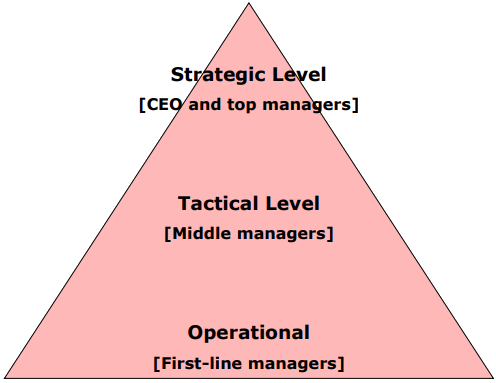
\includegraphics[scale=0.3]{figures/strategicallevel.png}
\caption{STO model}
\end{wrapfigure}

\noindent We identified the key problem to be located at the strategical level. Making Rasmus Hartung (CEO) the key problem owner as he has the influence, money and trust from investors to implement the required proposed solutions.\newline

\noindent Gunnar Brabrand the sales director shares the blame with not onborading new customers and Mads Dørup CTO shares the blame with the maintenance employee of not realising the need for maintenance help at tactical level. \color{red} rewrite \color{black} 
